% Options for packages loaded elsewhere
\PassOptionsToPackage{unicode}{hyperref}
\PassOptionsToPackage{hyphens}{url}
\PassOptionsToPackage{dvipsnames,svgnames,x11names}{xcolor}
%
\documentclass[
  letterpaper,
  DIV=11,
  numbers=noendperiod]{scrartcl}

\usepackage{amsmath,amssymb}
\usepackage{iftex}
\ifPDFTeX
  \usepackage[T1]{fontenc}
  \usepackage[utf8]{inputenc}
  \usepackage{textcomp} % provide euro and other symbols
\else % if luatex or xetex
  \usepackage{unicode-math}
  \defaultfontfeatures{Scale=MatchLowercase}
  \defaultfontfeatures[\rmfamily]{Ligatures=TeX,Scale=1}
\fi
\usepackage{lmodern}
\ifPDFTeX\else  
    % xetex/luatex font selection
\fi
% Use upquote if available, for straight quotes in verbatim environments
\IfFileExists{upquote.sty}{\usepackage{upquote}}{}
\IfFileExists{microtype.sty}{% use microtype if available
  \usepackage[]{microtype}
  \UseMicrotypeSet[protrusion]{basicmath} % disable protrusion for tt fonts
}{}
\makeatletter
\@ifundefined{KOMAClassName}{% if non-KOMA class
  \IfFileExists{parskip.sty}{%
    \usepackage{parskip}
  }{% else
    \setlength{\parindent}{0pt}
    \setlength{\parskip}{6pt plus 2pt minus 1pt}}
}{% if KOMA class
  \KOMAoptions{parskip=half}}
\makeatother
\usepackage{xcolor}
\setlength{\emergencystretch}{3em} % prevent overfull lines
\setcounter{secnumdepth}{-\maxdimen} % remove section numbering
% Make \paragraph and \subparagraph free-standing
\makeatletter
\ifx\paragraph\undefined\else
  \let\oldparagraph\paragraph
  \renewcommand{\paragraph}{
    \@ifstar
      \xxxParagraphStar
      \xxxParagraphNoStar
  }
  \newcommand{\xxxParagraphStar}[1]{\oldparagraph*{#1}\mbox{}}
  \newcommand{\xxxParagraphNoStar}[1]{\oldparagraph{#1}\mbox{}}
\fi
\ifx\subparagraph\undefined\else
  \let\oldsubparagraph\subparagraph
  \renewcommand{\subparagraph}{
    \@ifstar
      \xxxSubParagraphStar
      \xxxSubParagraphNoStar
  }
  \newcommand{\xxxSubParagraphStar}[1]{\oldsubparagraph*{#1}\mbox{}}
  \newcommand{\xxxSubParagraphNoStar}[1]{\oldsubparagraph{#1}\mbox{}}
\fi
\makeatother


\providecommand{\tightlist}{%
  \setlength{\itemsep}{0pt}\setlength{\parskip}{0pt}}\usepackage{longtable,booktabs,array}
\usepackage{calc} % for calculating minipage widths
% Correct order of tables after \paragraph or \subparagraph
\usepackage{etoolbox}
\makeatletter
\patchcmd\longtable{\par}{\if@noskipsec\mbox{}\fi\par}{}{}
\makeatother
% Allow footnotes in longtable head/foot
\IfFileExists{footnotehyper.sty}{\usepackage{footnotehyper}}{\usepackage{footnote}}
\makesavenoteenv{longtable}
\usepackage{graphicx}
\makeatletter
\newsavebox\pandoc@box
\newcommand*\pandocbounded[1]{% scales image to fit in text height/width
  \sbox\pandoc@box{#1}%
  \Gscale@div\@tempa{\textheight}{\dimexpr\ht\pandoc@box+\dp\pandoc@box\relax}%
  \Gscale@div\@tempb{\linewidth}{\wd\pandoc@box}%
  \ifdim\@tempb\p@<\@tempa\p@\let\@tempa\@tempb\fi% select the smaller of both
  \ifdim\@tempa\p@<\p@\scalebox{\@tempa}{\usebox\pandoc@box}%
  \else\usebox{\pandoc@box}%
  \fi%
}
% Set default figure placement to htbp
\def\fps@figure{htbp}
\makeatother
% definitions for citeproc citations
\NewDocumentCommand\citeproctext{}{}
\NewDocumentCommand\citeproc{mm}{%
  \begingroup\def\citeproctext{#2}\cite{#1}\endgroup}
\makeatletter
 % allow citations to break across lines
 \let\@cite@ofmt\@firstofone
 % avoid brackets around text for \cite:
 \def\@biblabel#1{}
 \def\@cite#1#2{{#1\if@tempswa , #2\fi}}
\makeatother
\newlength{\cslhangindent}
\setlength{\cslhangindent}{1.5em}
\newlength{\csllabelwidth}
\setlength{\csllabelwidth}{3em}
\newenvironment{CSLReferences}[2] % #1 hanging-indent, #2 entry-spacing
 {\begin{list}{}{%
  \setlength{\itemindent}{0pt}
  \setlength{\leftmargin}{0pt}
  \setlength{\parsep}{0pt}
  % turn on hanging indent if param 1 is 1
  \ifodd #1
   \setlength{\leftmargin}{\cslhangindent}
   \setlength{\itemindent}{-1\cslhangindent}
  \fi
  % set entry spacing
  \setlength{\itemsep}{#2\baselineskip}}}
 {\end{list}}
\usepackage{calc}
\newcommand{\CSLBlock}[1]{\hfill\break\parbox[t]{\linewidth}{\strut\ignorespaces#1\strut}}
\newcommand{\CSLLeftMargin}[1]{\parbox[t]{\csllabelwidth}{\strut#1\strut}}
\newcommand{\CSLRightInline}[1]{\parbox[t]{\linewidth - \csllabelwidth}{\strut#1\strut}}
\newcommand{\CSLIndent}[1]{\hspace{\cslhangindent}#1}

\KOMAoption{captions}{tableheading}
\makeatletter
\@ifpackageloaded{caption}{}{\usepackage{caption}}
\AtBeginDocument{%
\ifdefined\contentsname
  \renewcommand*\contentsname{Table of contents}
\else
  \newcommand\contentsname{Table of contents}
\fi
\ifdefined\listfigurename
  \renewcommand*\listfigurename{List of Figures}
\else
  \newcommand\listfigurename{List of Figures}
\fi
\ifdefined\listtablename
  \renewcommand*\listtablename{List of Tables}
\else
  \newcommand\listtablename{List of Tables}
\fi
\ifdefined\figurename
  \renewcommand*\figurename{Figure}
\else
  \newcommand\figurename{Figure}
\fi
\ifdefined\tablename
  \renewcommand*\tablename{Table}
\else
  \newcommand\tablename{Table}
\fi
}
\@ifpackageloaded{float}{}{\usepackage{float}}
\floatstyle{ruled}
\@ifundefined{c@chapter}{\newfloat{codelisting}{h}{lop}}{\newfloat{codelisting}{h}{lop}[chapter]}
\floatname{codelisting}{Listing}
\newcommand*\listoflistings{\listof{codelisting}{List of Listings}}
\makeatother
\makeatletter
\makeatother
\makeatletter
\@ifpackageloaded{caption}{}{\usepackage{caption}}
\@ifpackageloaded{subcaption}{}{\usepackage{subcaption}}
\makeatother

\usepackage{bookmark}

\IfFileExists{xurl.sty}{\usepackage{xurl}}{} % add URL line breaks if available
\urlstyle{same} % disable monospaced font for URLs
\hypersetup{
  pdftitle={Research Report on the Clorox Company},
  pdfkeywords={Financial Report, Feduciary},
  colorlinks=true,
  linkcolor={blue},
  filecolor={Maroon},
  citecolor={Blue},
  urlcolor={Blue},
  pdfcreator={LaTeX via pandoc}}


\title{Research Report on the Clorox Company}
\author{Andrey Malyukov \and Roza Bass}
\date{}

\begin{document}
\maketitle
\begin{abstract}
In September 2021, a significant jump in seismic activity on the island
of La Palma (Canary Islands, Spain) signaled the start of a volcanic
crisis that still continues at the time of writing. Earthquake data is
continually collected and published by the Instituto Geográphico
Nacional (IGN). \ldots{}
\end{abstract}

\renewcommand*\contentsname{Table of contents}
{
\hypersetup{linkcolor=}
\setcounter{tocdepth}{3}
\tableofcontents
}

\subsection{TODO}\label{todo}

Use ``PerformanceAnalytics'' package for Sharpe ratio and risk analysis.

Cite your stuff: (Regenstein 2020).

\subsection{Introduction}\label{introduction}

\section{}\label{section}

That's a nice intro.

\pandocbounded{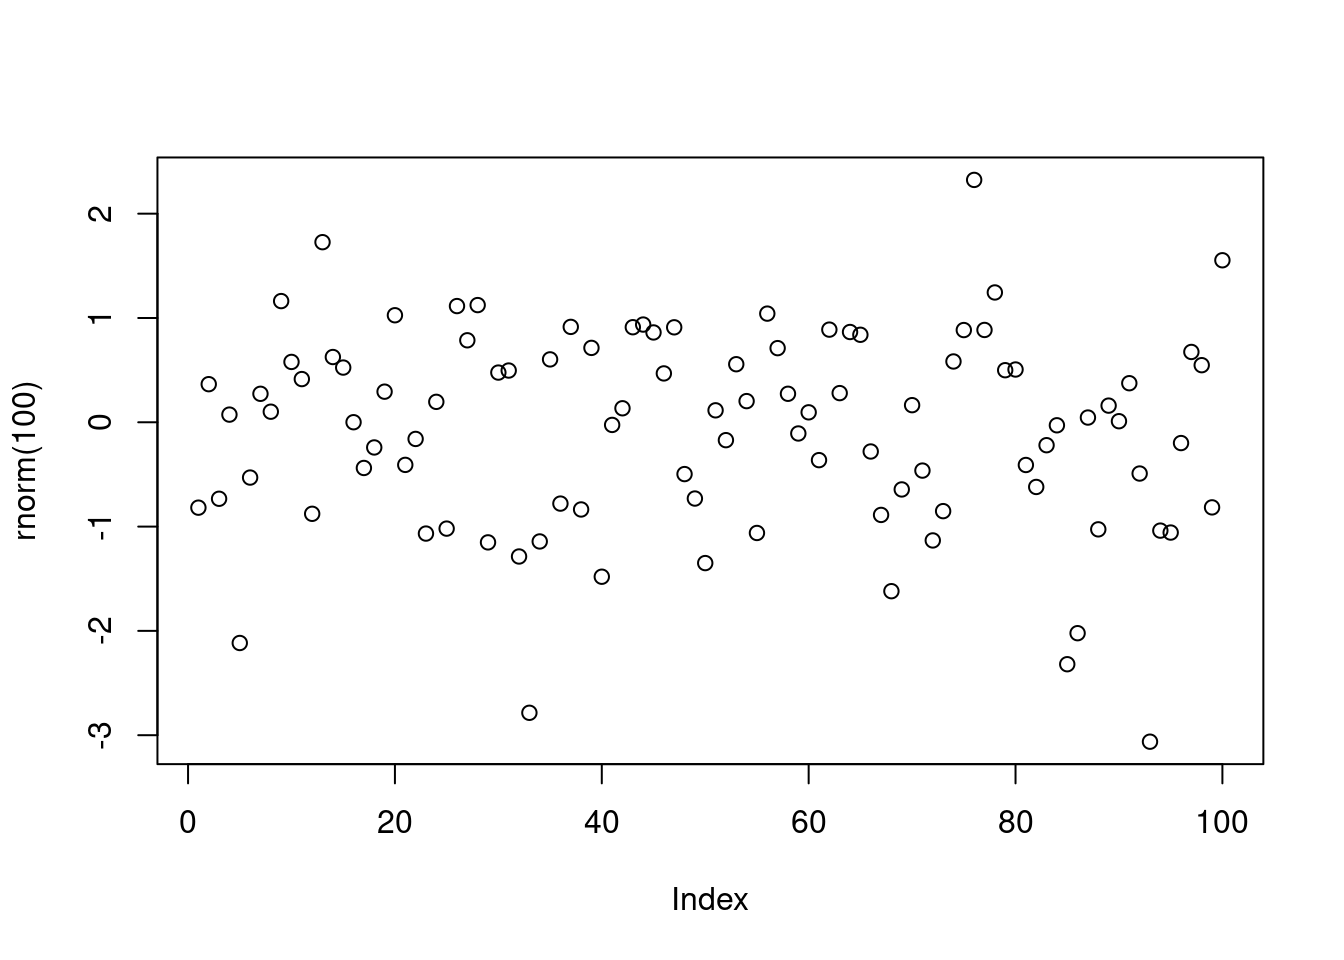
\includegraphics[keepaspectratio]{index_files/figure-latex/notebooks-intro-cell-2-output-1.png}}

We need better stuff though.

\begin{verbatim}
[1] "CPALTT01USQ657N"           CPALTT01USQ657N
1955-04-01       0.0000000
1955-07-01       0.4993758
1955-10-01       0.1242236
1956-01-01      -0.2481390
1956-04-01       0.8706468
1956-07-01       1.2330456     Index            CPALTT01USQ657N  
 Min.   :1955-04-01   Min.   :-2.8285  
 1st Qu.:1972-06-08   1st Qu.: 0.3950  
 Median :1989-08-16   Median : 0.8018  
 Mean   :1989-08-16   Mean   : 0.8959  
 3rd Qu.:2006-10-24   3rd Qu.: 1.1939  
 Max.   :2024-01-01   Max.   : 3.9508  
\end{verbatim}

\begin{table}

\caption{\label{tbl-planets}Astronomical object}

\centering{

\subcaption{\label{tbl-planets-1}}

\centering{

\pandocbounded{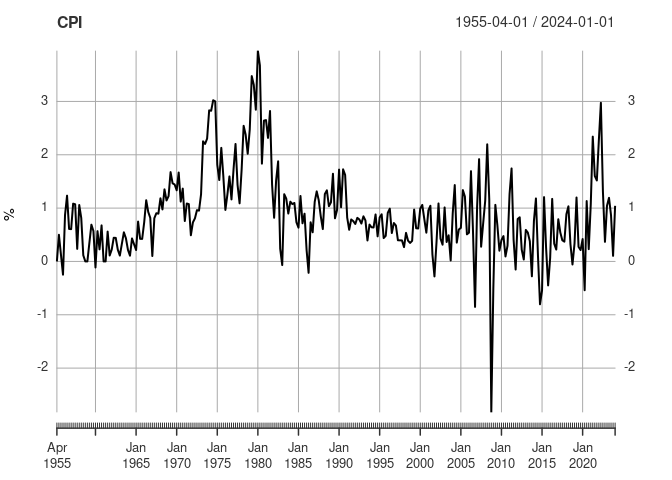
\includegraphics[keepaspectratio]{index_files/figure-latex/notebooks-intro-tbl-planets-output-3.png}}

}

}

\end{table}%

Use this kind of macroeconomic analysis maybe?

\subsection{Sector Analysis}\label{sector-analysis}

Performance of all sectors relative to each other.

https://alphaarchitect.com/2020/01/visualization-sector-trends-with-r-code/

Maybe that's a bit much.

\section{}\label{section-1}

\subsubsection{Financial Analysis of The Clorox Company (CLX) in the
Consumer Staples
Sector}\label{financial-analysis-of-the-clorox-company-clx-in-the-consumer-staples-sector}

\paragraph{\texorpdfstring{\textbf{1. GICS Sector
Classification}}{1. GICS Sector Classification}}\label{gics-sector-classification}

Clorox operates in the \textbf{Consumer Staples sector} (GICS 30),
specifically within the Household Products sub-industry. This sector is
characterized by stable demand, recession resilience, and brands focused
on essential goods like cleaning products, personal care items, and food
.

\begin{center}\rule{0.5\linewidth}{0.5pt}\end{center}

\paragraph{\texorpdfstring{\textbf{2. Position Relative to
Competitors}}{2. Position Relative to Competitors}}\label{position-relative-to-competitors}

Clorox competes with major players such as \textbf{Procter \& Gamble
(PG)}, \textbf{Colgate-Palmolive (CL)}, \textbf{Church \& Dwight (CHD)},
and \textbf{Kimberly-Clark (KMB)}. Key comparisons include:

\begin{longtable}[]{@{}
  >{\raggedright\arraybackslash}p{(\linewidth - 8\tabcolsep) * \real{0.1781}}
  >{\raggedright\arraybackslash}p{(\linewidth - 8\tabcolsep) * \real{0.1918}}
  >{\raggedright\arraybackslash}p{(\linewidth - 8\tabcolsep) * \real{0.2192}}
  >{\raggedright\arraybackslash}p{(\linewidth - 8\tabcolsep) * \real{0.2192}}
  >{\raggedright\arraybackslash}p{(\linewidth - 8\tabcolsep) * \real{0.1918}}@{}}
\toprule\noalign{}
\begin{minipage}[b]{\linewidth}\raggedright
\textbf{Metric}
\end{minipage} & \begin{minipage}[b]{\linewidth}\raggedright
\textbf{Clorox (CLX)}
\end{minipage} & \begin{minipage}[b]{\linewidth}\raggedright
\textbf{Colgate-Palmolive (CL)}
\end{minipage} & \begin{minipage}[b]{\linewidth}\raggedright
\textbf{Procter \& Gamble (PG)}
\end{minipage} & \begin{minipage}[b]{\linewidth}\raggedright
\textbf{Industry Avg}
\end{minipage} \\
\midrule\noalign{}
\endhead
\bottomrule\noalign{}
\endlastfoot
\textbf{Revenue (FY24)} & \$7.09B & \$20.10B & \$84.04B & Varies by
sub-industry \\
\textbf{Net Margin} & 6.38\% & 14.38\% & \textasciitilde18\% (est.) &
\textasciitilde10-15\% \\
\textbf{P/E Ratio} & 40.62 & 24.39 & 26.66 & 20-25 \\
\textbf{Dividend Yield} & 3.3\% & 2.3\% & 2.4\% & 2.5-3.5\% \\
\end{longtable}

\begin{itemize}
\tightlist
\item
  \textbf{Strengths}: Strong brands (e.g., Clorox bleach, Glad bags),
  ESG focus (recyclable packaging by 2025) .
\item
  \textbf{Weaknesses}: Lower profitability vs.~peers, cyberattack
  recovery costs .
\item
  \textbf{Market Share}: \textasciitilde1.99\% in cleaning products,
  lagging behind P\&G and Colgate .
\end{itemize}

\begin{center}\rule{0.5\linewidth}{0.5pt}\end{center}

\paragraph{\texorpdfstring{\textbf{3. Economic Indicator
Comparison}}{3. Economic Indicator Comparison}}\label{economic-indicator-comparison}

Clorox's performance relative to the \textbf{S\&P 500} and \textbf{Dow
Jones Industrial Average (DJIA)} highlights its defensive nature: -
\textbf{Beta}: 0.42 (less volatile than the market) . - \textbf{1-Year
Stock Performance}: -3.3\% (CLX) vs.~+7.9\% (S\&P 500) and +15.05\%
(DJIA) . - \textbf{Dividend Growth}: 35 consecutive years of increases,
outperforming many S\&P 500 staples .

\begin{center}\rule{0.5\linewidth}{0.5pt}\end{center}

\paragraph{\texorpdfstring{\textbf{4. Strategic and Financial
Challenges}}{4. Strategic and Financial Challenges}}\label{strategic-and-financial-challenges}

\begin{itemize}
\tightlist
\item
  \textbf{Cyberattack Impact}: Caused a 20\% Q1 FY24 sales decline,
  though recovery efforts restored \textasciitilde90\% market share by
  Q3 .
\item
  \textbf{Margin Recovery}: Gross margin expanded to 46.5\% in Q4 FY24,
  driven by cost savings .
\item
  \textbf{Divestitures}: Sold non-core businesses (Argentina, VMS) to
  focus on high-growth segments .
\end{itemize}

\begin{center}\rule{0.5\linewidth}{0.5pt}\end{center}

\paragraph{\texorpdfstring{\textbf{5. R Code for
Visualization}}{5. R Code for Visualization}}\label{r-code-for-visualization}

Below is R code to compare Clorox's stock performance with competitors
and indices:

\begin{verbatim}
[1] "CLX"
\end{verbatim}

\pandocbounded{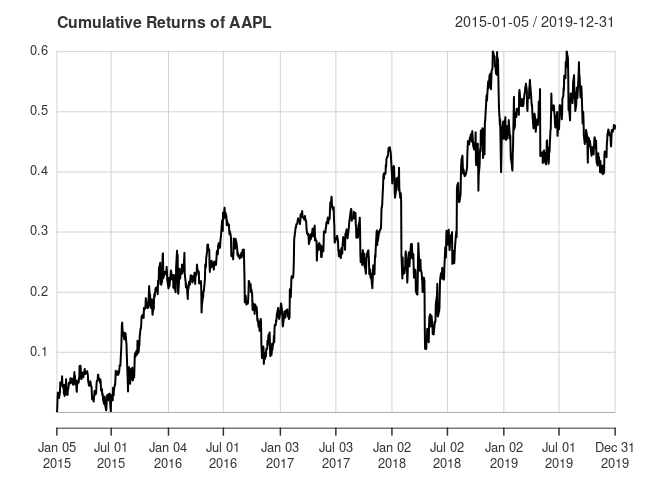
\includegraphics[keepaspectratio]{index_files/figure-latex/notebooks-sector-cell-2-output-3.png}}

\begin{center}\rule{0.5\linewidth}{0.5pt}\end{center}

\paragraph{\texorpdfstring{\textbf{6. Key
Insights}}{6. Key Insights}}\label{key-insights}

\begin{itemize}
\tightlist
\item
  Clorox's valuation (P/E 40.6) reflects optimism about its recovery and
  IGNITE strategy but is expensive compared to peers .
\item
  Consumer Staples sector growth (CAGR 3.7\% for cleaning products)
  supports long-term stability, but competition from eco-friendly brands
  (e.g., Seventh Generation) poses risks .
\item
  Clorox's underperformance vs.~indices highlights sector-specific
  challenges (inflation, supply chain) .
\end{itemize}

\begin{center}\rule{0.5\linewidth}{0.5pt}\end{center}

For real-time data, update the R code with current ticker prices and
adjust the date range. The analysis underscores Clorox's resilience in a
defensive sector but signals caution due to margin pressures and
competitive headwinds.

\subsection{Personality of the
Company}\label{personality-of-the-company}

\section{}\label{section-2}

\subsection{Fundamental Analysis}\label{fundamental-analysis}

\section{}\label{section-3}

\subsection{Technical Analysis}\label{technical-analysis}

\section{}\label{section-4}

\subsection{Company Performance
2019-2024}\label{company-performance-2019-2024}

\section{}\label{section-5}

\subsection{Forecasting}\label{forecasting}

\section{}\label{section-6}

\begin{itemize}
\tightlist
\item
  What risks does it list on 10-k? Summarize.
\end{itemize}

\pandocbounded{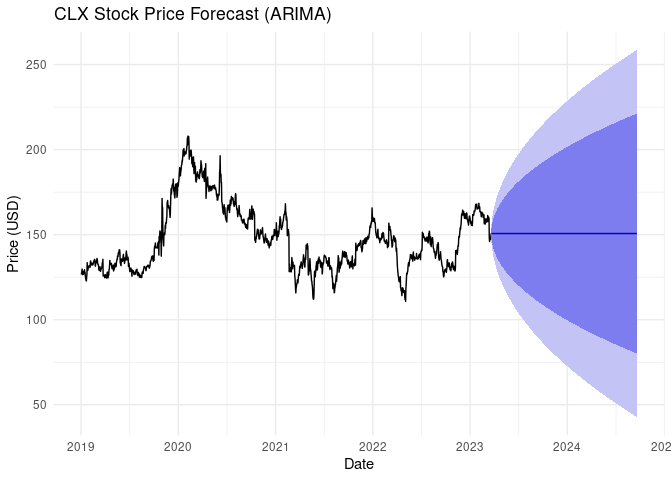
\includegraphics[keepaspectratio]{index_files/figure-latex/notebooks-forecasting-cell-2-output-2.png}}

\subsection{Summary}\label{summary}

\section{}\label{section-7}

\phantomsection\label{refs}
\begin{CSLReferences}{1}{0}
\bibitem[\citeproctext]{ref-regensteinVisualizationSectorTrends2020}
Regenstein, Jonathan. 2020. {``Visualization {Sector Trends} with {R
Code}.''} \emph{Alpha Architect}.
https://alphaarchitect.com/2020/01/visualization-sector-trends-with-r-code/.

\end{CSLReferences}




\end{document}
